\subsection{Степень устойчивости, запас устойчивости по 	фазе и амплитуде, их определение с помощью амплитудно-фазовых частотных характеристик или ЛАЧХ и ФЧХ непрерывной 	системы}

В условиях эксплуатации параметры системы по тем или иным причинам могут меняться в определенных пределах (старение, температурные колебания и т.п.). Эти колебания параметров могут привести к потере устойчивости системы, если она работает вблизи границы устойчивости. Поэтому стремятся спроектировать САУ так, чтобы она работала вдали от границы устойчивости. Степень этого удаления называют запасом устойчивости.

Согласно критерия Найквиста, чем дальше АФЧХ от критической точки (-1, j0), тем больше запас устойчивости. Различают запасы устойчивости по модулю и по фазе.

Запас устойчивости по модулю характеризует удаление годографа АФЧХ разомкнутой САУ от критической точки в направлении вещественной оси и определяется расстоянием h от критической точки до точки пересечения годографом оси абсцисс (левый рисунок).

Запас устойчивости по фазе характеризует удаление годографа от критической точки по дуге окружности единичного радиуса и определяется углом  между отрицательным направлением вещественной полуоси и лучом, проведенным из начала координат в точку пересечения годографа с единичной окружностью.

\begin{figure}[!h]
    \centering
    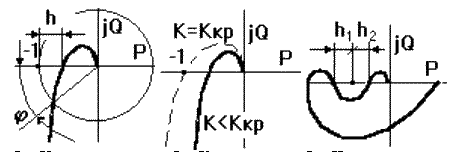
\includegraphics[width=0.5\textwidth]{images/stab.png}
    \caption{Поясняющие рисунки}
    \label{fig:stubs}
\end{figure}

Как уже отмечалось, с ростом коэффициента передачи разомкнутой САУ растет модуль каждой точки АФЧХ и при некотором значении K = Kкр АФЧХ пройдет через критическую точку (средний рисунок) и попадет на границу устойчивости, а при K > Kкр замкнутая САУ станет неустойчива. Однако в случае “клювообразных” АФЧХ (получаются из-за наличия внутренних обратных связей) не только увеличение, но и уменьшение K может привести к потере устойчивости замкнутых САУ (правый рисунок). В этом случае запас устойчивости определяется двумя отрезками h1 и h2, заключенными между критической точкой и АФЧХ.

Обычно при создании САУ задаются требуемыми запасами устойчивости h и, за пределы которых она выходить не должна. Эти пределы выставляются в виде сектора, вычерчиваемого вокруг критической точки, в который АФЧХ разомкнутой САУ входить не должна.


